\documentclass[12pt,a4paper]{article}
\usepackage[utf8]{inputenc}
\usepackage{amsmath}
\usepackage{blkarray}
\usepackage{amsfonts}
\usepackage{amssymb}
\usepackage{makeidx}
\usepackage{graphicx}
\usepackage{lmodern}
\usepackage{url}
\usepackage{color}
\usepackage[dvipsnames]{xcolor}
\usepackage{bm}
\usepackage{booktabs}
\usepackage{listings}
\usepackage[left=2cm,right=2cm,top=2cm,bottom=2cm]{geometry}
\author{Mudathir Mahgoub \\ 0119655301}
\title{Takehome Midterm Exam 2}
\begin{document}

\maketitle


\begin{enumerate}

\item Explain the differences between cross-site scripting (XSS) and cross-site
request forgery (CSRF) attacks in your own words. Describe a fictitious scenario in
which CSRF can be used to leak confidential information about the victim user. Finally,
explain the confused deputy problem in your own words. Give an example of a web
attack that occurs as the browser acts as the confused deputy.

\color{blue}

\color{black}

\item Explain the ``Spectre attack" in your own words and identify the goal of
the adversary for this attack. What is the fundamental weakness of the system that
the attackers exploit in the Spectre attack? What is the impact of the Spectre attack?
In your own words, give a scenario in which an attacker can exploit Spectre attack to
achieve something malicious.


\color{blue}

\color{black}

\item How does the different cryptographic currency schemes (e.g., Bitcoin) ensure
that an arbitrary adversary cannot bundle up some arbitrary transactions to make a
block and add it to the blockchain? Explain the process in your own words. Why is it
the case that an attacker can double spend only if he possesses 51\% of the computing
power of the whole network? Explain how is it possible.


\color{blue}


\color{black}

\item Explain the buffer overflow attack. Your description of the attack should
include the weakness of the system that the adversary exploits, the objective of the
adversary in this attack, and the steps the adversary should take to carry out this
attack. Describe the different defenses (e.g., Canary, ASLR) that can thwart the buffer overflow attack, and discuss their relative advantages and disadvantages. Can you have buffer overflow attacks in a program written in Java? Please explain your answer.


\color{blue}

\color{black}

\item Suppose you are given the following C function $function\_to\_test (.,.)$ that
takes as input two integers $x$ and $y$, and returns another integer $z$. The function has a
bug denoted by the statement ``assert(0)".

\definecolor{light-gray}{gray}{0.97}
\lstset{ 
  backgroundcolor=\color{light-gray},   % choose the background color; you must add \usepackage{color} or \usepackage{xcolor}; should come as last argument
  basicstyle=\scriptsize,        % the size of the fonts that are used for the code  
  commentstyle=\color{ForestGreen},    % comment style    
  keywordstyle=\color{blue},       % keyword style
  language=C,                 % the language of the code  
  numbers=left,                    % where to put the line-numbers; possible values are (none, left, right)
  numbersep=5pt,                   % how far the line-numbers are from the code
  numberstyle=\tiny\color{red}, % the style that is used for the line-numbers 
  tabsize=2	                   % sets default tabsize to 2 spaces 
}

\begin{lstlisting} 
int function_to_test(int x, int y) {
	/*Suppose inputs x and y are set to have symbolic values */
	
	int k = x - y;
	int t = x + y + 3;
	if(x % 2 == 0) /* check whether x is even; remainder is 0 when x is divisible by 2 */
	{
		x = y + 1;
		++y; /* Increment y value by 1 */
		if(t > 0){
			k = t - 2;
		}
	}	
	if(x+6 > k) {
		y = 5;
	}
	if(t+x+y == 20){ /* Check whether t+x+y is equal to 20*/
		assert(0); /* Bug */
	}
	
	int z = (t + x + y) / x; 
	return z;
}
\end{lstlisting}

\begin{enumerate}
\item Your goal is to run symbolic execution on the following program and determine which concrete inputs for the variables $x$ and $y$ trigger the bug.

\color{blue}

\color{black}

\item Please show all the path constraints resulting due to the symbolic execution on the following program.

\color{blue}
\begin{figure}[h]
 \centering
 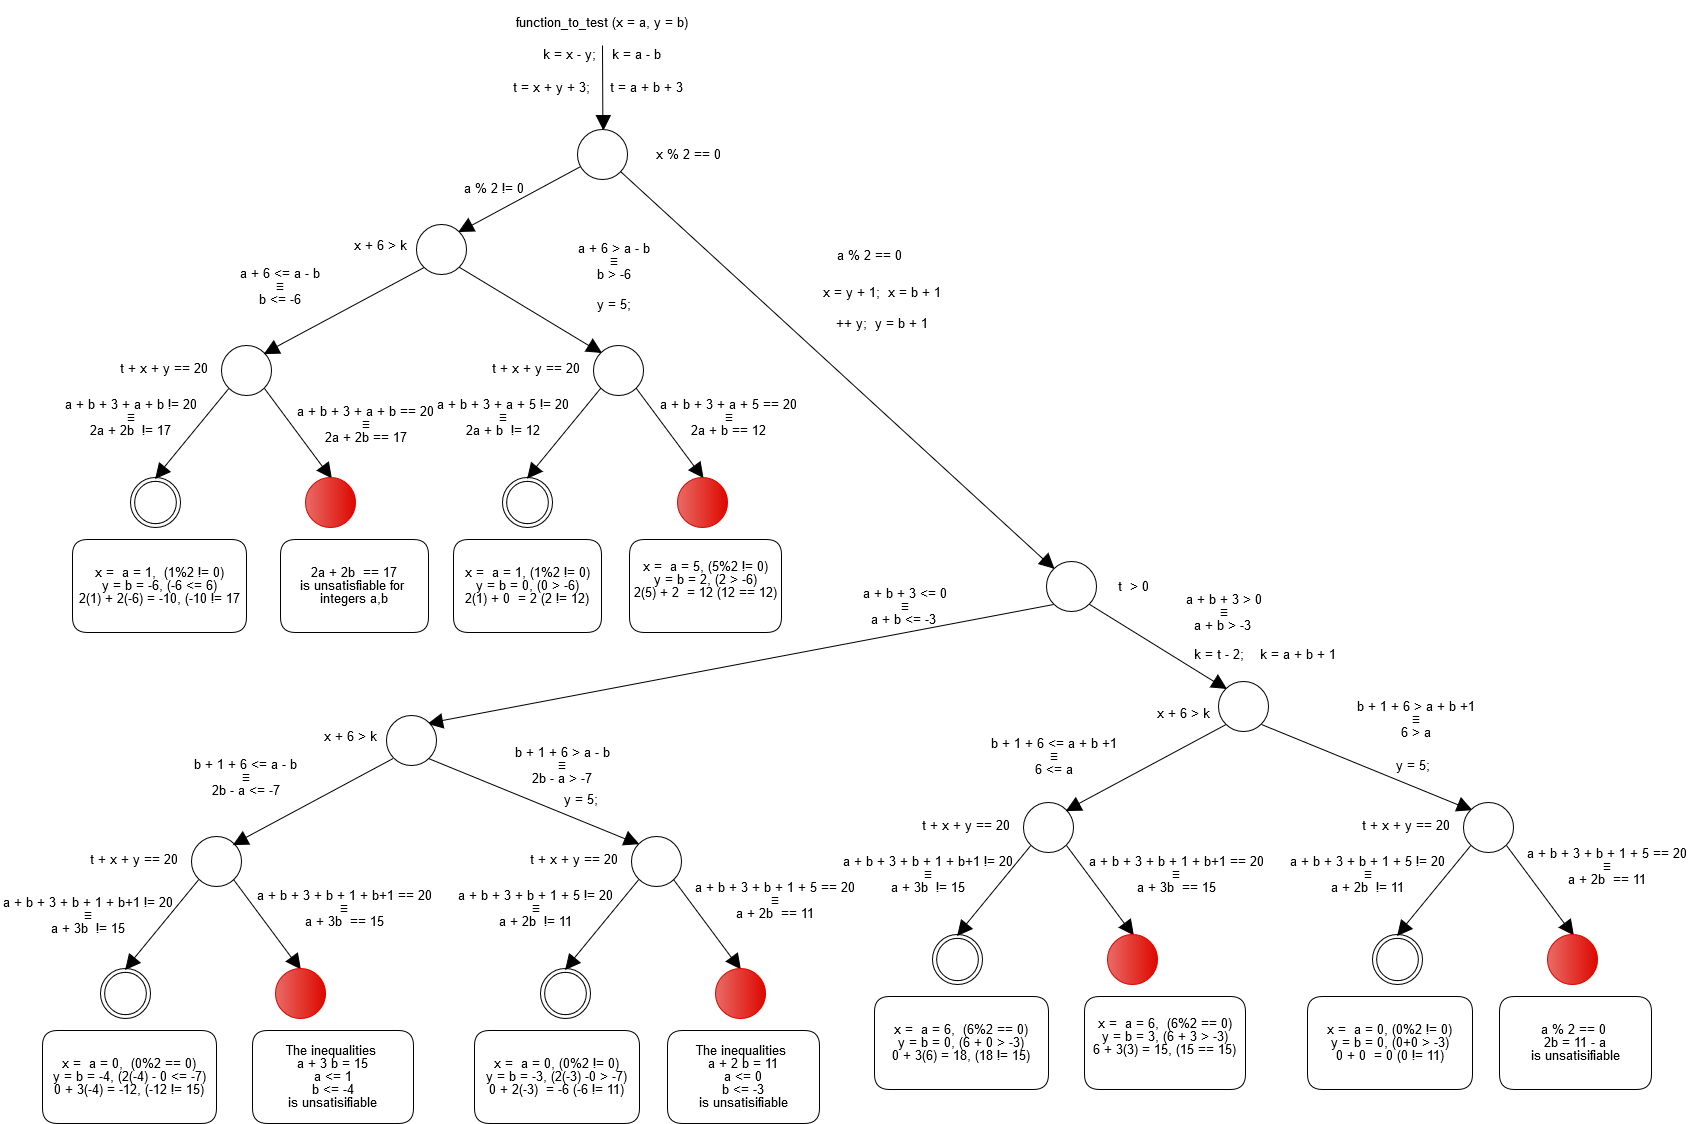
\includegraphics[scale=.25,keepaspectratio=true]{./paths.png}
\end{figure}
\color{black}

\item Additionally, assume that you would like the symbolic execution to identify whether the function has any ``divide by zero" exceptions. How would you modify the symbolic execution to identify such cases?
 \color{black}

\item Provide the modified path constraints due to the additional divide by zero checking.
\color{blue}

\color{black}

\item Explain what would change if you were to use concolic execution instead of symbolic execution
while answering sub-question (a) described above.

\color{blue}

\color{black}

\end{enumerate}
\end{enumerate}

\end{document}
